\section{Distributed development}
In the highly competitive services marketplace, businesses are seeking new ways to take advantage of labor arbitrage using a global resource pool -- to get services that are ``cheaper, better, faster''.  As the services market place has matured, it has become increasingly apparent that hap-hazard use of outsourcing is a double edged sword -- traditional project management techniques do not scale well to a global workforce, unless they are supplemented by an over-arching organizational and procedural structure suitable for supporting distributed teams of practitioners.

Distributed development and its implicit challenges have become the norm in recent years and this phenomenon has received a lot of interest~\cite{glo24,glo26}. The nature of these challenges has been analyzed in recent literature. Evaristo~\cite{glo27} categorizes them into five critical areas: Perceived distance (geographical and temporal), National culture (languages, accepted work patterns), Development methodology (similarity in processes), Task structure (clarity and structure to team hand-offs) and Organizational distance. The premise is that as the distance between the teams along these critical dimensions increases, the overhead and difficulties associated with distributed development become more prominent.

Collaborative development platforms that promote structured interaction between team members can help make distributed development more efficient~\cite{glo28,glo29}. Sharing expertise and the ability to leverage best practices across engagements is a key part of ensuring efficient collaboration – Expertise Browser~\cite{glo30} and Hipikat~\cite{glo31} are examples of tools that enable sharing at the level of processes and artifacts. Given the rapid churn of resources in the global workforce, a push model of delivering information in situ to developers is important and many of the proposed tools~\cite{glo29,glo31,glo34} support this model.

Formal process modeling, strict enforcement of process controls and monitoring the software development process have long been touted as the right way to streamline global delivery~\cite{glo32,glo33,glo34}. Using capability maturity models as a way to rate the operational maturity of an organization has been in vogue for many years and has been widely adopted by the industry~\cite{glo35}. Milos~\cite{glo34} provides a structured approach to instrumenting processes and tasks.

\subsection{Competency center models}
The last few years have seen an accelerated trend towards organizations utilizing a globally integrated development (GID) model for complex IT solution implementation. As with other services, in the first wave of the move towards globally integrated development, the emphasis was on reducing the cost structure through labor arbitrage.  The competition among the major industry players generated the need for aggressive differentiation that goes beyond the benefits of lower cost -- improving quality and reducing time-to-market are becoming key differentiators. In practice, traditional project management techniques that worked well with small co-located teams do not seem to scale well to a global workforce. Practical experience shows that unless development process adopted for GID should be supplemented by an over-arching procedural and architectural framework, that implicitly partitions the development process, it will not be effective.

As GID matured a second wave of IT services innovation lead to the adoption of software development and deployment practices that improve quality and increase productivity while preserving the advantages of labor arbitrage.  The adoption of a disciplined model for delivery by GID has resulted in new organizational efficiencies, reduced process variance and execution discipline. Figure~\ref{glofig1}, shows the vision of the globally integrated enterprise by focusing on one of the key pain points that inhibit this vision – a structured way of distributing work to remote teams that promotes collaboration and enforces good governance practices.  Some of the key organizational entities in this approach include: governance and operations teams, a design center that builds the architecture in support of client requirements, and the technology assembly centers which deliver the work. IBM has been a pioneer in this field -- their approach to structured delivery of IT services by a globally distributed delivery team is called application assembly optimization (AAO)~\cite{gloaao}. Other major IT services companies have adopted variations of this same approach.

\begin{figure}[h]
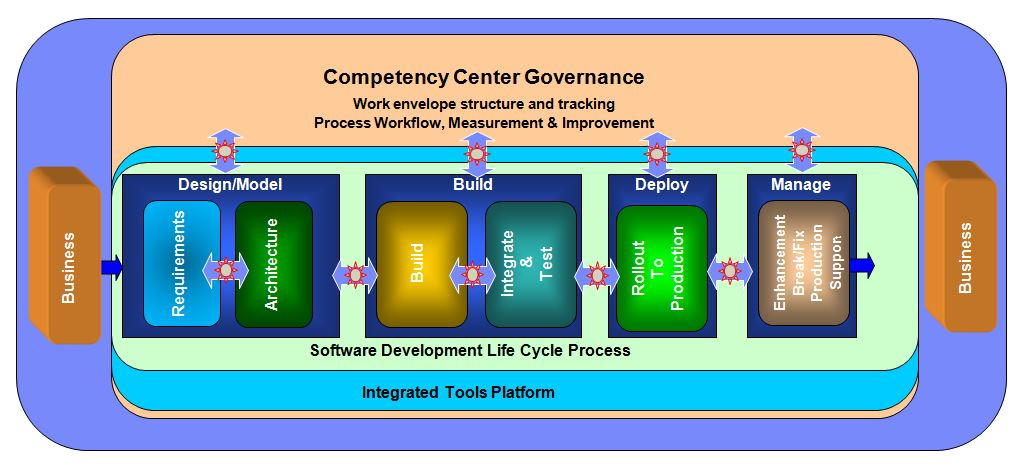
\includegraphics[scale=0.2]{figs/glocomp.jpg}
\caption{GID model with competency centers}
\label{glofig1}
\end{figure}

Work envelopes are central constructs in this approach to structured delivery of software projects that enable disparate technology assembly centers to come together on-demand in the context of a client engagement.  The work envelopes represent a standard envelope by which every work order is authored, transported, and delivered. Work packets include workflow, instruction (normative guidance), metrics collection, and risk management/exception handling mechanisms. Each work envelope constitutes a sub-set of activities that are bound to a larger project plan WBS managed through a traditional project management (PM) tool. Figure~\ref{glo-fig2} shows an example organization of a work envelope.

\begin{figure}[h]
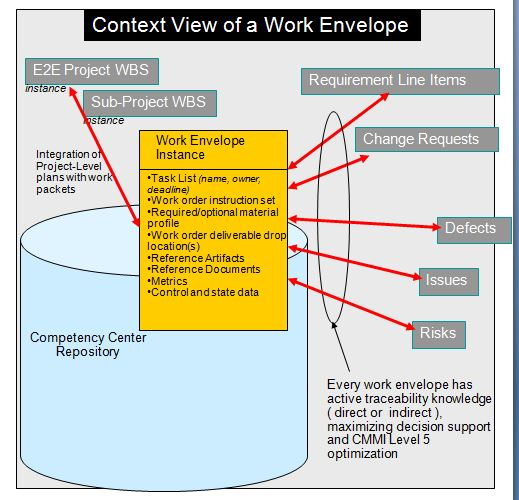
\includegraphics[scale=0.2]{figs/glowenv.jpg}
\caption{Work Envelope}
\label{glofig2}
\end{figure}

The goals of organizing delivery in this fashion include offering expert guidance through structured work envelopes that reduce training time and mentoring, consistent workflow through its governance of process execution and deliverable handoffs, and detailed tracking through timely and accurate windows into task status across globally distributed teams for improved performance and continuous improvement. This approach assumes many of the foundational elements of an organization, and therefore needs governance which integrates into existing governance models at the client IT shop.

\subsection{Towards distributed marketplaces}

As GID becomes common place, the ability to modularize work itself so each chunk could be distributed between any one of a set of distributed providers becomes critical. This is the logical evolution of the competency center model that we discussed in the last section. In essence, we propose the concept of a competitive services marketplace.  The realization of such a marketplace is enabled by two core concepts: (1) provide the mechanism to compete for work by matching the provider’s capabilities to the consumer’s requirements, and (2) a fool-proof measurement system that grades providers on their ability to meet/exceed their commitments. Instances of such marketplaces are already appearing - for example, services that provide coding expertise for hire such as RentACoder (www.rentacoder.com), TopCoder (www.topcoder.com) are early examples. Currently, they are seen as a novelty and thus have gained little adoption in large enterprises. However, we strongly feel that with the appropriate coordination and governance mechanisms in place a truly global marketplace can play a significant role in providing an efficient alternative to traditional IT vendors.

 A services delivery marketplace has three key players: provider, consumer and a marketplace enabler. The consumer can use the enabler to ascertain the risks that he is taking in sourcing from a particular provider. The provider in turn gets the ability to competitively price his services based on his delivery record. The enabler provides core enabling services such as: decomposing large or complex projects so they can be executed in parallel by different providers, managing complex projects that are executed in parallel by different providers, providing service level guarantees, or performing service request validation. It is important to note that our marketplace concept is itself an abstraction for efficient service delivery. Thus, all three players can belong to the same organization, each be a different organization in the true global-marketplace sense, or any combination thereof. 
 
 Traditional IT vendors still play a role in this conceptual services marketplace -- however, small or marginal players also have a chance to compete and grow their reputation. In this setup, there are incentives for every one to participate. For traditional IT vendors, it helps offload low margin IT services to smaller vendors with less overhead. For customers it gives an opportunity to out source small work without entering into expensive long term contracts. For the marketplace providers -- who we think will be traditional IT vendors -- it is a chance to profit from helping both providers and consumers take advantage of the marketplace by offering some guarantees.
 
 The primary goal of a service delivery marketplace, is to provide managed delivery of services with a carefully crafted and monitored agreement between the consumer and the provider. In contrast to a marketplace for complete products, service delivery is inherently more challenging as it is difficult to capture the intent of the consumer when a service request is created. The service request should not only set forth the details of the work that is to be performed but also make provision to clearly specify risk mitigation, change management, periodic reviews, documentation requirements and exit criteria in a clear fashion to set the right expectations for both the consumer and the provider.  For example, if a code development project being worked on by a provider is not progressing as per the agreed upon schedule agreed upon, a risk mitigation activity may even involve canceling the service agreement. Unless such a risk mitigation activity is clearly spelled out during the creation of the service request, it may open up avenues for misunderstanding. Figure~\ref{glomarketplace} shows the conceptual instantiation of such a marketplace.
 
 \begin{figure}[h]
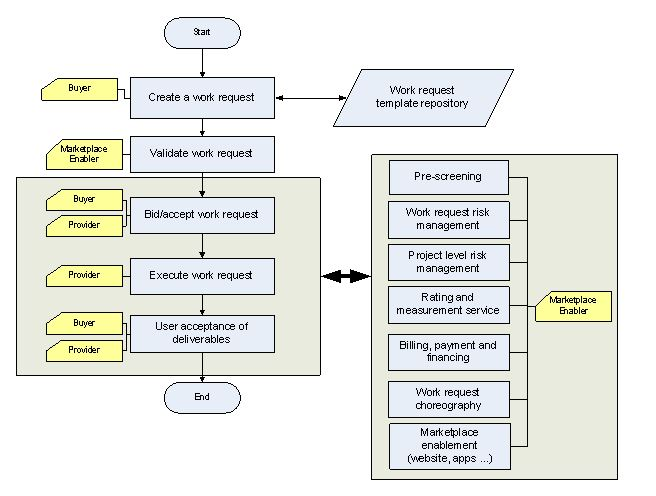
\includegraphics[scale=0.4]{figs/glomarketplace.jpg}
\caption{Services Marketplace}
\label{glomarketplace}
\end{figure}
 
 To make this concept practical there are many challenges to be overcome. The primary challenge is reducing the overhead required to partition and distribute a large software project into independent units of work that can be done by skilled developers with little or no reference to the overall project context. Packaged applications, for example those provided by SAP and Oracle, may provide the most opportunities in the beginning. However, even complex custom software may be developed by a distributed workforce without prohibitive coordination costs. Open source software development is a case in point where complex software has been developed through a very loosely organized set of developers. For large enterprises, this mode of development may not be suitable as it does not offer appropriate security, governance and schedule controls. 
 
 Theoretical analysis can point to optimal regimes and controls for the efficient use of a services marketplace. Ranade and Varshney~\cite{glo-ranade} use game theoretic models to offer key insights into some key questions about crowd sourcing in general:what type of tasks should be crowd sourced under what circumstances? Their conclusion depending on the types of tasks (specialized vs generic) and the distribution of skills in the available pool of people will have a big impact on the types of tasks that can be outsourced.

\label{sec:global}



